\newcommand{\valuecom}[1]{\textcolor{green!60!black}{/\!/ #1}}
\newcommand{\textdom}[1]{\mathsf{#1}}
\newcommand{\textcode}[1]{\texorpdfstring{\texttt{#1}}{#1}}
\newcommand{\kw}[1]{\textbf{\textcode{#1}}}
\newcommand{\skipc}{\kw{skip}}
\newcommand{\ite}[3]{\kw{if}\;#1\:\kw{then}\;#2\;\\ \kw{else}\;#3}
\newcommand{\iteml}[3]{
  \kw{if} \; #1\\
  \begin{array}[t]{@{}l@{}l}
    \kw{then}& \begin{array}[t]{l} #2 \end{array} \\
    \kw{else}& \begin{array}[t]{l} #3 \end{array} \\
  \end{array}
}

\newcommand{\set}[1]{\{{#1}\}}
\newcommand{\defeq}{\triangleq}
\renewcommand{\implies}{\Rightarrow}

\colorlet{colorPO}{gray!60!black}
\colorlet{colorRF}{green!60!black}
\colorlet{colorMO}{orange}
\colorlet{colorFR}{purple}
\colorlet{colorECO}{red!80!black}
\colorlet{colorSYN}{green!40!black}
\colorlet{colorHB}{blue}
\colorlet{colorPPO}{magenta}
\colorlet{colorPB}{olive}
\colorlet{colorSBRF}{olive}
\colorlet{colorRMW}{olive!70!black}
\colorlet{colorRSEQ}{blue}
\colorlet{colorSC}{violet}
\colorlet{colorPSC}{violet}
\colorlet{colorREL}{olive}
\colorlet{colorCONFLICT}{olive}
\colorlet{colorRACE}{olive}
\colorlet{colorWB}{orange!70!black}
\colorlet{colorPSC}{violet}
\colorlet{colorSCB}{violet}
\colorlet{colorDEPS}{violet}
\colorlet{colorAR}{black}

\tikzset{
   every path/.style={>=stealth},
   po/.style={->,color=colorPO,thin,shorten >=-0.5mm,shorten <=-0.5mm},
   sw/.style={->,color=colorSYN,shorten >=-0.5mm,shorten <=-0.5mm},
   rf/.style={->,color=colorRF,dashed,,shorten >=-0.5mm,shorten <=-0.5mm},
   hb/.style={->,color=colorHB,thick,shorten >=-0.5mm,shorten <=-0.5mm},
   co/.style={->,color=colorMO,dotted,very thick,shorten >=-0.5mm,shorten <=-0.5mm},
   no/.style={->,dotted,thick,shorten >=-0.5mm,shorten <=-0.5mm},
   fr/.style={->,color=colorFR,dotted,thick,shorten >=-0.5mm,shorten <=-0.5mm},
   deps/.style={->,color=colorDEPS,dotted,thick,shorten >=-0.5mm,shorten <=-0.5mm},
   rmw/.style={->,color=colorRMW,thick,shorten >=-0.5mm,shorten <=-0.5mm},
   pngexport/.style={
     external/system call/.add=
     {}
     {; convert -density 300 -transparent white "\image.pdf" "\image.png"},
     % 
     /pgf/images/external info,
     /pgf/images/include external/.code={%
       \includegraphics
       [width=\pgfexternalwidth,height=\pgfexternalheight]
       {##1.png}%
     },
   }
 }
\newcommand{\dpo}[2]{\draw[po] (#1) edge (#2)}
\newcommand{\dpopo}[2]{\draw[po] (#1) edge node[right] {$\lPO$} (#2)}
\newcommand{\drmw}[2]{\draw[rmw, bend right=20] (#1) edge node[left] {$\lRMW$} (#2)}
\newcommand{\dco}[2]{\draw[co] (#1) edge node[right] {$\lCO$} (#2)}
\newcommand{\dcoext}[4]{\draw[co, #3] (#1) edge node[#4] {$\lCO$} (#2)}
\newcommand{\drf}[2]{\draw[rf] (#1) edge node[left] {$\lRF$} (#2)}
\newcommand{\dfr}[3]{\draw[fr, #3] (#1) edge node[left] {$\lFR$}(#2)}
\newcommand{\dhb}[3]{\draw[hb, #3] (#1) edge node[right] {$\lHB$} (#2)}


%% Orders
\newcommand{\pln}{\mathtt{pln}}
\newcommand{\rlx}{\mathtt{rlx}}
\newcommand{\rel}{{\mathtt{rel}}}
\newcommand{\acq}{{\mathtt{acq}}}
\newcommand{\acqrel}{{\mathtt{acqrel}}}
\newcommand{\sco}{{\mathtt{sc}}}
% omm modes
\newcommand{\na}{{\mathtt{na}}}
\newcommand{\at}{{\mathtt{at}}}

%% Event labels
\newcommand{\rlab}[3]{{\lR}^{#1}({#2},{#3})}
\newcommand{\wlab}[3]{{\lW}^{#1}({#2},{#3})}
\newcommand{\flab}[1]{{\lF}(#1)}

\newcommand{\lR}{{\mathtt{R}}}
\newcommand{\lW}{{\mathtt{W}}}
\newcommand{\lF}{{\mathtt{F}}}
\newcommand{\lE}{{\mathtt{E}}}

%% Relations
\newcommand{\lPO}{{\color{colorPO}\mathtt{po}}}
\newcommand{\lRF}{{\color{colorRF} \mathtt{rf}}}
\newcommand{\lRMW}{{\color{colorRMW} \mathtt{rmw}}}
\newcommand{\lMO}{{\color{colorMO} \mathtt{mo}}}
\newcommand{\lMOx}{{\color{colorMO} \mathtt{mo}}_x}
\newcommand{\lMOy}{{\color{colorMO} \mathtt{mo}}_y}
\newcommand{\lCO}{{\color{colorMO} \mathtt{co}}}
\newcommand{\lCOx}{{\color{colorMO} \mathtt{co}}_x}
\newcommand{\lCOy}{{\color{colorMO} \mathtt{co}}_y}
\newcommand{\lFR}{{\color{colorFR} \mathtt{fr}}}
\newcommand{\lFRx}{{\color{colorFR} \mathtt{rb}}_x}
\newcommand{\lFRy}{{\color{colorFR} \mathtt{rb}}_y}
\newcommand{\lECO}{{\color{colorECO} \mathtt{eco}}}
\newcommand{\lSW}{{\color{colorSYN}\mathtt{sw}}}
\newcommand{\lHB}{{\color{colorHB}\mathtt{hb}}}
\newcommand{\lHBO}{{\color{olive}\mathtt{hbo}}}
\newcommand{\lDOB}{{\mathtt{dob}}}
\newcommand{\lBOB}{{\mathtt{bob}}}
\newcommand{\lAOB}{{\mathtt{aob}}}
\newcommand{\lOBS}{{\mathtt{obs}}}
\newcommand{\lEORD}{{\mathtt{eord}}}
\newcommand{\lTORD}{{\mathtt{tord}}}
\newcommand{\lSC}{{\mathtt{sc}}}
\newcommand{\lAR}{{\color{colorAR} \mathtt{ar}}}

\newcommand{\lSCB}{{\color{colorSCB} \mathtt{scb}}}
\newcommand{\lPSC}{{\color{colorPSC} \mathtt{psc}}}
\newcommand{\lPSCB}{\lPSC_{\rm base}}
\newcommand{\lPSCF}{\lPSC_\lF}

\newcommand{\lDEPS}{{{\color{colorDEPS}\mathtt{deps}}}}
\newcommand{\lCTRL}{{{\color{colorDEPS}\mathtt{ctrl}}}}
\newcommand{\lCTRLISYNC}{{{\color{colorDEPS}\mathtt{ctrl_{isync}}}}}
\newcommand{\lDATA}{{{\color{colorDEPS}\mathtt{data}}}}
\newcommand{\lADDR}{{{\color{colorDEPS}\mathtt{addr}}}}
\newcommand{\lCASDEP}{{{\color{colorDEPS}\mathtt{casdep}}}}

\newcommand{\lmakeE}[1]{#1\mathtt{e}}
\newcommand{\lRFE}{\lmakeE{\lRF}}
\newcommand{\lCOE}{\lmakeE{\lCO}}
\newcommand{\lFRE}{\lmakeE{\lFR}}
\newcommand{\lMOE}{\lmakeE{\lMO}}
\newcommand{\lmakeI}[1]{#1\mathtt{i}}
\newcommand{\lRFI}{\lmakeI{\lRF}}
\newcommand{\lCOI}{\lmakeI{\lCO}}
\newcommand{\lFRI}{\lmakeI{\lFR}}

\newcommand{\Tid}{\mathsf{Tid}}
\newcommand{\Loc}{\mathsf{Loc}}
\newcommand{\Val}{\mathsf{Val}}
\newcommand{\Init}{\mathsf{Init}}
\newcommand{\Lab}{\mathsf{Lab}}
\newcommand{\Mod}{\mathsf{Mod}}
\newcommand{\Modr}{\mathsf{Mod}_{\lR}}
\newcommand{\Modw}{\mathsf{Mod}_{\lW}}
\newcommand{\Modf}{\mathsf{Mod}_{\lF}}
\newcommand{\Modrmw}{\mathsf{Mod}_{\lU}}


% example rels
\newcommand{\exX}{\mathtt{x}}
\newcommand{\exY}{\mathtt{y}}

\definecolor{StringRed}{rgb}{.637,0.082,0.082}
\definecolor{CommentGreen}{rgb}{0.0,0.55,0.3}
\definecolor{KeywordBlue}{rgb}{0.0,0.3,0.55}
\definecolor{LinkColor}{rgb}{0.55,0.0,0.3}
\definecolor{CiteColor}{rgb}{0.55,0.0,0.3}
\definecolor{HighlightColor}{rgb}{0.0,0.0,0.0}

\definecolor{grey}{rgb}{0.5,0.5,0.5}
\definecolor{red}{rgb}{1,0,0}
\definecolor{darkgreen}{rgb}{0.0,0.7,0.0}

\hypersetup{%
  linktocpage=true, pdfstartview=FitV,
  breaklinks=true, pageanchor=true, pdfpagemode=UseOutlines,
  plainpages=false, bookmarksnumbered, bookmarksopen=true, bookmarksopenlevel=3,
  hypertexnames=true, pdfhighlight=/O,
}


\newcommand{\commentNonempty}[1]{
  \ifx\\#1\\
    {}
  \else
    \valuecom{#1}
  \fi
  }
\newcommand{\readInst}[4]{#1 \;:=\;[#2]^{#4}; \commentNonempty{#3}}
\newcommand{\fenceInst}[1]{\mathtt{fence}^{#1};}
\newcommand{\writeInst}[3]{[#1]^{#3}\;:=\;#2;}
\newcommand{\casInstSC}[3]{\mathtt{CAS^{\sco, \sco}_{\sco}(#1, #2, #3)};}
\newcommand{\assignInst}[2]{#1\;:=\;#2;}
\newcommand{\exchangeInstSC}[2]{\mathtt{exchange^{\sco}(#1, #2)};}
\newcommand{\term}[1]{\emph{#1}}



\newcommand{\Wrlx}{\lW^{\rlx}}
\newcommand{\Rrlx}{\lR^{\rlx}}
\newcommand{\Wsc}{\lW^{\sco}}
\newcommand{\Rsc}{\lR^{\sco}}
\newcommand{\Fa}{\lF^{\acq}}
\newcommand{\Fr}{\lF^{\rel}}
\newcommand{\Far}{\lF^{\acqrel}}
\newcommand{\ar}{\ensuremath{ar}}
\newcommand{\IMM}{\mathtt{IMM}}
\newcommand{\OMM}{\mathtt{OCaml}\allowbreak \mathtt{MM}}
\newcommand{\todo}[1]{\textbf{\Large TODO: \textcolor{red}{#1}}}
\newcommand{\strongereq}{\sqsupseteq}
\newcommand{\defin}[1]{\textit{#1}}
\newcommand{\imm}{|_{imm}}

%%% Local Variables:
%%% mode: latex
%%% TeX-master: t
%%% End:



\hyphenation{%
  не-сог-ла-со-ван-ность
}

% \begin{document}

% \filltitle{ru}{
%     chair              = {Кафедра системного программирования},
%     title              = {Компиляция модели памяти OCaml в Power},
%     type               = {master},
%     position           = {студента},
%     group              = 18.М08-мкн,
%     author             = {Намаконов Егор Сергеевич},
%     supervisor         = {Кознов Д.\,В.},
%     supervisorPosition = {д.ф.-м.н.},
%     reviewer           = {Березун Д. А.},
%     reviewerPosition   = {к.ф.-м.н.},
%     consultant         = {Подкопаев А.В.},
%     consultantPosition = {к.ф.-м.н.},
%     % chairHead          = {Хунта К.\,Х.},
%     % chairHeadPosition  = {д.\,ф.-м.\,н., профессор},
%   university         = {Санкт-Петербургский государственный университет},
%   faculty            = {Математическое обеспечение и администрирование информационных систем},
%   city               = {Санкт-Петербург},
%   year               = {2020}
% }
% \filltitle{en}{
%     chair              = {Software Engineering},
%     title              = {Compilation of OCaml memory model to Power},
%     author             = {Egor Namakonov},
%     supervisorPosition = {D. Sc.},
%     supervisor         = {Dmitri Koznov},
%     consultant         = {Anton Podkopaev},
%     consultantPosition = {Ph.D.},
%     reviewer           = {Daniil Berezun},
%     reviewerPosition   = {Ph.D.},
%     faculty            = {Software and Administration of Information Systems},
%     % chairHeadPosition  = {professor},
%     % chairHead          = {Christobal Junta},
% }

% \maketitle

% % \begin{abstract}
% % \end{abstract}
% % {\bf Ключевые слова:} слабые модели памяти, корректность компиляции, многопоточность.
% \newgeometry{a4paper,top=20mm,bottom=20mm,left=30mm,right=15mm,nohead,includeheadfoot} % for some reason it's ignored when placed in cls file

\tableofcontents



\section{Введение}

Результат исполнения многопоточной программы, как правило, является недетерминированным. Конкретное множество допустимых результатов многопоточной программы определяется \defin{моделью памяти} языка программирования. Наиболее известной является   \defin{модель последовательной согласованности} (\foreignlanguage{english}{sequential consistency}, SC \cite{sc}). Она предполагает, что любой результат исполнения программы может быть получен путём попеременного исполнения инструкций отдельных потоков согласно программному порядку в них. Однако из-за оптимизаций, выполняемых современными компиляторами и процессорами, могут наблюдаться сценарии поведения, невозможные в такой модели. Так, на архитектуре x86 чтение по адресу в памяти может вернуть не самое последнее записанное значение, так как операция записи может быть буферизована. 

Отказ от подобных оптимизаций нежелателен, поэтому современные модели памяти допускают некоторые сценарии поведения, невозможные в модели SC. Такие модели памяти называются \defin{слабыми}. Например, слабыми являются модели памяти языков C++ \cite{cpp}, JavaScript \cite{js-mm} и Java \cite{jmm}, а также архитектур Power \cite{power}, x86 \cite{x86} и ARM \cite{arm}.

%Как правило, слабые модели памяти дают более сильные гарантии на поведение программ, в которых конфликтующие обращения по одному и тому же адресу должным образом синхронизированы. В противном случае такие обращения образуют \defin{гонку по данным}, и в этом случае модель памяти может ослабить гарантии на поведение программы. Так, в модели C++ к гонке по данным приводят конфликтующие неатомарные обращения, и в этом случае поведение всей программы объявляется неопределённым \cite{cpp}.
%В модели памяти Java для предотвращения гонки используются встроенные в язык средства синхронизации \cite{jmm}; в случае же возникновения гонки по некоторому адресу допускается чтение произвольных значений по нему в будущем \cite{omm}.

%Для обеспечения баланса между производительностью и предсказуемостью поведения программы современные модели памяти предоставляют программисту гарантии DRF (data race freedom, \textit{свобода от гонок}). Они гарантируют, что поведение программы, не содержащей гонок по данным, будет согласовано с моделью SC. Например, свойство DRF предоставляют модели памяти Java и Promising \cite{promising}. 

Модель памяти OCaml \cite{omm} (далее --- $\OMM$) отличается свойством т.н.  \textit{локальной свободы от гонок по данным} (local data race freedom). Именно, гарантируется, что выполнение конфликтующих обращений по выбранному адресу в памяти (т.е. ситуация гонки по данным) не влияет на обращения к другим адресам, а также на последующие обращения по тому же адресу. Благодаря этому даже при возникновении гонки по данным в некоторый момент исполнения следующие участки программы будут исполнены согласно модели SC. 

% Для того, чтобы использовать $\OMM$ на практике, необходимо доказать её реализуемость на распространённых архитектурах процессоров.
Чтобы гарантировать выполнение этого свойства, при компиляции нужно запретить некоторые оптимизации в зависимости от целевой архитектуры.
% Этого можно достичь, если в зависимости от типа инструкции при компиляции выбирать подходящие режимы доступа или добавлять барьеры в ассемблерный код.
Для этого может понадобиться, например, добавить в ассемблерный код инструкции-\defin{барьеры}, которые запрещают нежелательные оптимизации на уровне процессора. 
Набор таких правил, покрывающий все возможные типы инструкций, называется \defin{схемой компиляции}. Схема компиляции должна быть \defin{корректной} --- при исполнении любой программы, полученной при компиляции согласно этой схеме, должно наблюдаться только сценарии поведения, разрешённые $\OMM$ для исходной программы.

Авторы $\OMM$ разработали схемы компиляции $\OMM$ в модели x86-TSO и ARMv8 \cite{omm} и доказали их корректность. При этом отсутствует схема компиляции в модель архитектуры Power. А между тем данная архитектура часто используется в современном серверном оборудовании \cite{power-servers}. Задача построения такой схемы осложнена тем, что модель Power, в отличие от моделей x86-TSO, ARMv8 и $\OMM$, не обладает т.н. свойством \defin{multicopy atomicity}. Такое свойство означает, что записанные в память значения становятся доступны всем потокам в одном и том же порядке \cite{arm}. Из-за отсутствия этого свойства корректная схема компиляции $\OMM$ в Power должна расставлять барьеры в результирующей программе так, чтобы запретить нежелательные сценарии поведения. 

В рамках данной работы была поставлена задача разработать схему компиляции $\OMM$ в модель Power и доказать её корректность. Для этого было решено использовать промежуточную модель памяти (Intermediate Memory Model, далее — $\IMM$) \cite{imm}, для которой уже доказана корректность компиляции в модель Power. Использование $\IMM$ как промежуточного этапа компиляции позволяет разбить доказательство корректности  на два, которые впоследствии можно использовать в других доказательствах. Таким образом, построение схемы компиляции $\OMM$ в $\IMM$ даёт схемы компиляции $\OMM$ не только в Power, но и другие архитектуры, в которые компилируется $\IMM$ (на данный момент --- x86 и ARM). 


\section{Постановка задачи}

Целью данной работы является доказательство корректности компиляции модели памяти OCaml ($\OMM$) в модель памяти Power \cite{power}. 

В работе были поставлены следующие задачи:

\begin{itemize}
\item построение схемы компиляции $\OMM$ в $\IMM$ (для которой корректность компиляции в Power уже доказана);
\item доказательство корректности полученной схемы;
\item формализация доказательства в системе интерактивного доказательства теорем Coq \cite{coq-description}.
\end{itemize}

\section{Обзор}

В этом разделе приводится пример слабого поведения программы и объясняются его причины. Затем на примерах рассматривается понятие корректности компиляции для моделей памяти. Далее формально описывается декларативный способ задания модели памяти \cite{power}, основанный на понятии графов исполнения. Наконец, формально описываются модели памяти $\OMM$ и $\IMM$, используемые далее в работе.

\subsection{Пример исполнения в слабой модели памяти}

Рассмотрим программу, представленную на \cref{fig:store-buffering}. Здесь и далее используется упрощённый синтаксис программ: $x$ и $y$ обозначают адреса в памяти, $a$ и $b$ — локальные переменные (регистры), $\rlx$ – режим доступа (это понятие будет рассмотрено ниже). Сверху указаны изначальные значения в памяти. В комментариях указаны наблюдаемые при чтении значения. Согласно модели SC, в зависимости от порядка исполнения инструкций в $a$ и $b$ могут быть записаны значения $(1, 1)$, $(1, 0)$ или $(0, 1)$. Однако после компиляции C++-аналога этой программы с помощью компилятора gcc и исполнения на архитектуре x86 в переменные $a$ и $b$ могут быть записаны нули, что не допускается моделью SC. У такого сценария поведения могут быть две причины. Во-первых, gcc может поменять местами обращения по разным адресам во время компиляции. Во-вторых, при исполнении на x86 возможна буферизация записи: в целях оптимизации обращений к памяти запись может быть отложена. 

\begin{figure}[h]
  \centering
  \begin{tabular}{l || l}
    \multicolumn{2}{c}{$x = 0,\ y = 0$} \\
    \hline
    $\writeInst{x}{1}{\rlx}$ & $\writeInst{y}{1}{\rlx}$ \\
    $\readInst{a}{y}{0}{\rlx}$ & $\readInst{b}{x}{0}{\rlx}$ \\
  \end{tabular}
  \caption{Пример программы и её исполнения при буферизации записи}
  \label{fig:store-buffering}
\end{figure}

% Стоит отметить, что после оптимизации некоторых обращений к памяти поведение программы может перестать соответствовать спецификации.
Новые сценарии поведения программы, возникающие в результате оптимизаций, могут быть некорректными с точки зрения требований к программе. Поэтому слабая модель памяти должна предоставлять возможность отменить оптимизации для отдельных инструкций. Для этого используются \defin{режимы доступа}, различные по степени строгости.
% В зависимости от режима доступа инструкции при её компиляции могут быть отменены оптимизации, а также добавлены дополнительные инструкции-\defin{барьеры}, которые запрещают оптимизации на уровне процессора.
% Компилятор по-разному обрабатывает инструкции с разными режимами доступа; в частности, перед отдельными инструкциями могут быть
При компиляции инструкций с более строгими режимами компилятор может отменить некоторые оптимизации, а также добавить в результирующую программу инструкции-барьеры. 

Так, в программе на \cref{fig:store-buffering} был использован режим доступа $\rlx$, который не ограничивает оптимизации соответствующих инструкций. Модель памяти C++ гарантирует, что если в этой программе для всех инструкций установить режим доступа $\sco$ вместо $\rlx$, то поведение полученной программы будет согласовано с моделью SC. Это справедливо в силу того, что  такие обращения будут скомпилированы с использованием инструкции MFENCE \cite{cpp-mappings} --- барьера памяти, запрещающего перестановки SC инструкций.

\subsection{Проблема корректности компиляции на примерах} \label{corr-comp-example}

Модели $\OMM$ и $\IMM$ определены декларативно \cite{power}. Это означает, что каждое возможное поведение программы задаётся в виде \defin{графа исполнения}, а семантика программы определяется как множество графов, удовлетворяющих некоторому условию. Пример программы и одного из графов её исполнения приведён на \cref{fig:example-discriminating}.

%Метки $\na$ и $\at$ в программе на \cref{fig:example-discriminating} обозначают \defin{режимы доступа} соответствующих инструкций. Режимы доступа назначаются программистом для отмены оптимизаций отдельных инструкций. Так, запись в режиме $\at$ на архитектуре x86 компилируется\cite{omm} в инструкцию атомарной замены \texttt{xchg}, перед исполнением которой буфер записей очищается, что ограничивает множество возможных поведений программы.

Вершины графа соответствуют событиям --- операциям над разделяемой памятью, которые производятся при выполнении инструкций программы. Так, событие $\lW^{\at}(x, 1)$ соответствует записи по адресу $x$ значения $1$ в режиме $\at$; другими типами событий являются чтение и барьер памяти (обозначаются $\lR$ и $\lF$ соответственно). Кроме того, в графе выделяются инициализирующие события, которые соответствуют инициализирующей записи нулей в память. На \cref{fig:example-discriminating} все они для краткости обозначены множеством $\mathtt{Init}$; далее в графах мы будем опускать эти события, если это не будет важно для рассуждений. Заметим, что содержимое локальных переменных потока не отражается в графе в явном виде, т.к. взаимодействие между потоками производится только через разделяемую память. 

\begin{figure}[h]
  \centering
  \begin{minipage}{0.45\textwidth}
    \centering
    \begin{tabular}{l || l || l}
      \multicolumn{3}{c}{$\writeInst{x}{0}{}\ \writeInst{y}{0}{}$} \\
      \hline
      $\writeInst{x}{1}{\at}$ & $\readInst{a}{x}{1}{\at}$ & $\readInst{b}{y}{1}{\na}$ \\
      {}            & $\writeInst{y}{1}{\na}$ & $\readInst{c}{x}{0}{\at}$ \\
    \end{tabular}
  \end{minipage}\hfill
  \begin{minipage}{0.45\textwidth}
    \centering
    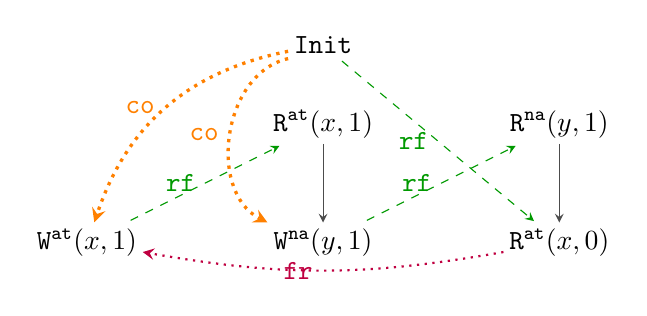
\begin{tikzpicture}[yscale=1,xscale=1]
      \node (Winit) at (3,1) {$\mathtt{Init}$};
      
      \node (T1W1) at (0, -1.5) {$\wlab{\at}{x}{1}$};
      \dcoext{Winit}{T1W1}{bend right=30}{left};
      
      \node (T2R1) at (3,0) {$\rlab{\at}{x}{1}$};
      \drf{T1W1}{T2R1};
      \node (T2W1) at (3, -1.5) {$\wlab{\na}{y}{1}$};
      \dpo{T2R1}{T2W1};
      \dcoext{Winit}{T2W1}{bend right=70}{left};
      
      \node (T3R1) at (6,0) {$\rlab{\na}{y}{1}$};
      \drf{T2W1}{T3R1};
      \node (T3R2) at (6,-1.5) {$\rlab{\at}{x}{0}$};
      \dpo{T3R1}{T3R2}; 
      \drf{Winit}{T3R2};
      \dfr{T3R2}{T1W1}{bend left=10};
    \end{tikzpicture}
  \end{minipage}
  \caption{Пример программы и сценария её исполнения, не согласованного в $\OMM$}
  \label{fig:example-discriminating}
\end{figure}

Рёбра графа задают бинарные отношения между событиями. В данном графе есть четыре
различных отношения: рёбра $\lPO$ соответствуют программному порядку инструкций, $\lRF$ --- чтению записанного ранее значения, $\lCO$ --- порядку выполнения записи по одному адресу, $\lFR$ --- чтению до указанного события записи. Отношения $\lPO$ и $\lCO$ являются транзитивными, поэтому для их задания достаточно указывать только непосредственные рёбра. Кроме того, для краткости будем опускать подпись $\lPO$ рядом с соответствующими рёбрами.

\defin{Согласованными} (допустимыми моделью) называются те сценарии исполнения программы, графы которых удовлетворяют некоторому предикату, заданному моделью. В частности, предикат согласованности $\OMM$ требует, чтобы в графе не было циклов, состоящих только из рёбер $\lCO$ и $\lFR$, проходящих между вершинами с меткой $\at$, а также рёбер $\lPO$ и $\lRF$. Это условие формализует свойство multicopy atomicity, описанное выше.

Граф исполнения на \cref{fig:example-discriminating} не является согласованным по $\OMM$. Действительно, этот сценарий исполнения нарушает свойство multicopy atomicity: второй поток читает записанное в $x$ значение $1$ до записи $1$ в $y$, однако третий поток читает старое значение $0$ из $x$ после чтения $1$ из $y$. Соответствующий граф исполнения не удовлетворяет предикату согласованности $\OMM$, так как между вершинами есть цикл, подходящий под описание выше. Таким образом, в $\OMM$ после исполнения программы на \cref{fig:example-discriminating} переменные $a$, $b$ и $c$ не могут содержать значения $1$, $1$ и $0$ соответственно.

Условие корректности компиляции требует, чтобы сценарии поведения, запрещённые для исходной программы в $\OMM$, также были запрещены для скомпилированной программы в $\IMM$. Для декларативных моделей памяти это означает, что из несогласованности графа исполнения в $\OMM$ должна следовать несогласованность соответствующего ему графа исполнения  в $\IMM$. При этом, как будет показано далее, можно рассматривать вопрос согласованности по $\OMM$ только для графа исполнения скомпилированной программы.

На \cref{fig:example-imm-consistent} приведён результат компиляции программы на \cref{fig:example-discriminating} согласно тривиальной схеме компиляции. 
Такая схема лишь заменяет режимы инструкций на их аналоги в $\IMM$: $\na$ заменяется на $\rlx$, а $\at$ — на $\sco$; дополнительных инструкций не вводится. Соответственно, граф исполнения на \cref{fig:example-imm-consistent} отличается от графа на \cref{fig:example-discriminating} только метками вершин, и в нём сохраняется цикл того же вида. $\IMM$ не гарантирует свойство multicopy atomicity, и потому предикат её согласованности не требует отсутствия таких циклов. Поэтому граф на \cref{fig:example-imm-consistent} согласован, что делает соответствующий ему сценарий поведения разрешается $\IMM$, в отличие от $\OMM$. Поэтому тривиальная схема компиляции не является корректной.

\begin{figure}[h]
  \centering
  \begin{minipage}{0.45\textwidth}
    \centering
    \begin{tabular}{l || l || l}
      \multicolumn{3}{c}{$\writeInst{x}{0}{}\ \writeInst{y}{0}{}$} \\
      \hline
      $\writeInst{x}{1}{\sco}$ & $\readInst{a}{x}{1}{\sco}$ & $\readInst{b}{y}{1}{\rlx}$ \\
      {}            & $\writeInst{y}{1}{\rlx}$ & $\readInst{c}{x}{0}{\sco}$ \\
    \end{tabular}
  \end{minipage}\hfill
  \begin{minipage}{0.45\textwidth}
    \centering
    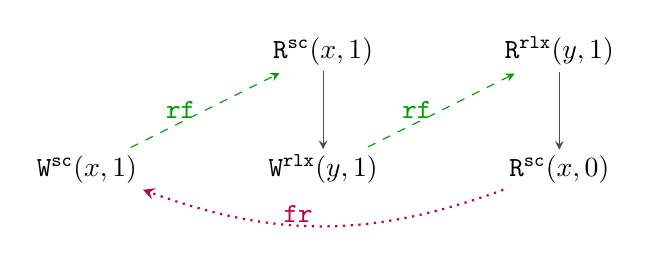
\begin{tikzpicture}[yscale=1,xscale=1]
      
      \node (T1W1) at (0, -1.5) {$\wlab{\sco}{x}{1}$};
      
      \node (T2R1) at (3,0) {$\rlab{\sco}{x}{1}$};
      \drf{T1W1}{T2R1};
      \node (T2W1) at (3, -1.5) {$\wlab{\rlx}{y}{1}$};
      \dpo{T2R1}{T2W1};
      
      \node (T3R1) at (6,0) {$\rlab{\rlx}{y}{1}$};
      \drf{T2W1}{T3R1};
      \node (T3R2) at (6,-1.5) {$\rlab{\sco}{x}{0}$};
      \dpo{T3R1}{T3R2}; 
      % \dfr{T3R2}{T1W1}{bend left=20};
      \draw[fr, bend left=20] (T3R2) edge node[left, yshift=1ex] {$\lFR$}(T1W1);
    \end{tikzpicture}
  \end{minipage}
  \caption{Результат компиляции программы на \cref{fig:example-discriminating} с использованием тривиальной схемы компиляции и согласованный по $\IMM$ граф его исполнения}
  \label{fig:example-imm-consistent}
\end{figure}

На \cref{fig:example-imm-inconsistent} приведена программа, полученная в результате компиляции программы на \cref{fig:example-discriminating} согласно схеме компиляции, приведённой в разделе \ref{compilation-scheme}. В результате компиляции в ней появляются инструкции барьеров памяти, запрещающие некоторые оптимизации процессора и компилятора. С этими барьерами граф исполнения перестаёт быть согласованным: из рёбер $\lRF$ между событиями с меткой $\sco$, а также $\lFR$, $\lPO$ и окружённого барьерами $\lRF$ образуется цикл, запрещённый в $\IMM$.


\newcommand{\vsIV}{-1.2}
\newcommand{\hsIV}{2.2}

\newcommand{\inconsistentExample}[1]{
      \begin{tikzpicture}[yscale=1,xscale=1]
      
      \node (T1F1) at (0, 0) {$\flab{\acq}$};
      \node (T1R1) at (0, \vsIV * 1) {$\rlab{\sco}{x}{0}$};
      \dpo{T1F1}{T1R1};
      \node (T1W1) at (0, \vsIV * 2) {$\wlab{\sco}{x}{1}$};
      \dpo{T1R1}{T1W1};
      \drmw{T1R1}{T1W1};
      
      \node (T2F1) at (\hsIV,0) {$\flab{\acq}$};
      \node (T2R1) at (\hsIV,\vsIV * 1) {$\rlab{\sco}{x}{1}$};
      \dpo{T2F1}{T2R1};
      \drf{T1W1}{T2R1};
      \node (T2F2) at (\hsIV,\vsIV * 2) {$\flab{\acqrel}$};
      \dpo{T2R1}{T2F2};
      \node (T2W1) at (\hsIV,\vsIV * 3) {$\wlab{\rlx}{y}{1}$};
      \dpo{T2F2}{T2W1};
      
      \node (T3R1) at (\hsIV * 2,0) {$\rlab{\rlx}{y}{1}$};
      \drf{T2W1}{T3R1};
      \node (T3F1) at (\hsIV * 2,\vsIV * 1) {$\flab{\acq}$};
      \dpo{T3R1}{T3F1};
      \node (T3R2) at (\hsIV * 2,\vsIV * 2) {$\rlab{\sco}{x}{0}$};
      \dpo{T3F1}{T3R2};
      % \dhb{T2F2}{T3F1}{bend right=5};
      \dfr{T3R2}{T1W1}{bend left=#1};
    \end{tikzpicture}
  }

\begin{figure}[!h]
%   % foobar
  % \centering
  \begin{minipage}{0.45\textwidth}
    % \centering
    \begin{tabular}{l || l || l}
      \multicolumn{3}{c}{$\writeInst{x}{0}{}\ \writeInst{y}{0}{}$} \\
      \hline
      $\fenceInst{\acq}$ & $\fenceInst{\acq}$ & $\readInst{b}{y}{1}{\rlx}$ \\
      $\exchangeInstSC{x}{1}$ & $\readInst{a}{x}{1}{\sco}$ & $\fenceInst{\acq}$\\
      {} & $\fenceInst{\acqrel}$ & $\readInst{c}{x}{0}{\sco}$\\
      {} & $\writeInst{y}{1}{\rlx}$ & {} \\
    \end{tabular}
    % bar
  \end{minipage} \hfill
  \begin{minipage}{0.45\textwidth}
    % \centering
    \inconsistentExample{70}
    % foo
  \end{minipage}

  % \caption{foobar}
  % \captionof{figure}{boofar}
  % \caption{Результат компиляции программы на \cref{fig:example-discriminating} с использованием схемы компиляции из раздела \ref{compilation-scheme} и его граф исполнения, не согласованный в $\IMM$}
  {\todo{Компиляция падает, если здесь использовать caption} Результат компиляции программы на \cref{fig:example-discriminating} с использованием схемы компиляции из раздела \ref{compilation-scheme} и его граф исполнения, не согласованный в $\IMM$}
  \label{fig:example-imm-inconsistent}    
\end{figure}

Таким образом, для доказательства корректности компиляции необходимо доказать
следующую теорему\footnote{Формальное понятие соответствие графов вводится в разделе \ref{compilation-scheme}.}.

\begin{restatable}{thm}{compiletheorem}
% \begin{definition}
  \label{prop:compile-theorem}
  Пусть $PO=||_{\tau\in \Tid} PO_\tau$ и $PI=||_{\tau\in \Tid} PI_\tau$ --- программы для моделей $\OMM$ и $\IMM$ соответственно, причём для любого $\tau \in \Tid$ подпрограмма $PI_\tau$ получена компиляцией $PO_\tau$ с помощью схемы компиляции из \cref{table:scheme}. Пусть $G_I$ --- согласованный по $\IMM$ граф исполнения $PI$. Тогда существует $G_O$ --- согласованный по $\OMM$ граф исполнения $PO$, соответствующий $G_I$. 
\end{restatable}


Ключевой идеей доказательства является то, что согласованность по $\OMM$ можно рассматривать для обоих графов исполнения. Для доказательства теоремы достаточно показать, что $G_I$ является согласованным по $\OMM$. Из этого следует согласованность $G_O$ по $\OMM$, так как он фактически является подграфом $G_I$ , а условия согласованности по $\OMM$ таковы, что выполняются для подграфов. Условие согласованности по $\OMM$ состоит в иррефлексивности одного отношения и ацикличности другого. Для каждого из этих отношений доказывается включение в такое отношение, для которого соответствующее условие выполняется в согласованном по $\IMM$ графе.

\subsection{Графы исполнения}
\label{exec-graphs}

В описаниях декларативных моделей памяти мы будем использовать следующие обозначения отношений между вершинами. Для бинарного отношения $R$ обозначения $R^?$, $R^{+}$, $R^{*}$ соответствуют его рефлексивному, транзитивному и транзитивно-рефлексивному замыканиям соответственно. Обратное отношение записывается как $R^{-1}$. Левая композиция отношений $R_1$ и $R_2$ записывается следующим образом:

$R_1;R_2 \defeq \set{x, y | \exists z. (x, z) \in R_1 \land (z, y) \in R_2}$.

Непосредственные рёбра $R$ обозначаются как $\imm R \defeq R \backslash R;R$. Тождественное отношение на множестве $A$ обозначается как $[A]$; в частности, $[A];R;[B] = R \cap (A \times B)$.

В данном разделе описываются графы исполнения наиболее общего вида, без привязки к конкретным моделям памяти или языкам. 

Считаем, что анализируемая программа $P$ состоит из последовательных подпрограмм отдельных потоков $P_\tau$: $P = ||_{\tau\in \Tid} P_\tau$, где $||$ --- оператор параллельной композиции программ, а $\Tid$ --- конечное множество идентификаторов потоков.

% \begin{definition}
\begin{restatable}{mydefinition}{graph}
  \emph{Граф исполнения} $G$ задаётся множеством вершин, бинарными отношениями на вершинах, а также функцией, сопоставляющей вершинами \emph{метки}. 
\end{restatable}
%\end{definition}
  
  Множество вершин, обозначаемое как $G.\lE$, делится на инициализирующие события вида $\mathtt{Init}\ loc$ и неинициализирующие события вида $\mathtt{ThreadEvent}\ \tau\ n$. Их компонентами являются:
  \begin{itemize}
  \item $loc \in \Loc$ --- адрес инициализации, где $\Loc$ --- конечное множество адресов;
  \item $\tau \in \Tid$ --- номер потока;
  \item $n\in \mathbb{N}$ --- порядковый номер внутри потока.
  \end{itemize}
    
Функция $G.\Lab$ сопоставляет событиям \term{метки} вида $(type, loc, mode, val)$. Их компонентами являются:
\begin{itemize}
\item $type \in \{\lR, \lW, \lF\}$ --- тип операции (чтение, запись, барьер);
\item $loc \in \Loc$ --- адрес памяти (для барьера не определено);
\item $mode$ --- один из режимов доступа (например, $\rel$), частично упорядоченных отношением ``строже чем'' ($\sqsubset$); конкретное множество режимов и их порядок определяется моделью памяти;
\item $val\in \Val$ --- прочитанное/записанное значение (в случае барьера не определено), где $\Val$ --- множество значений, которые могут храниться в памяти.
\end{itemize}

Следует отметить, что инициализирующие события вида $\mathtt{Init}\ loc$ обрабатываются особым образом. Именно,

$G.\Lab(\mathtt{Init}\ loc) = (\lW, loc, mode_{\Init}, val_{\Init})$, где $mode_{\Init}$ --- выбранный режим доступа для инициализирующих событий записей (например, в $\IMM$ --- $\rlx$), а $val_{\Init}$ --- начальное значение в памяти (как правило, 0).

Для множеств событий с определёнными метками вводятся соответствующие обозначения. Например, события с меткой чтения в режиме $\acq$ или более строгим будем обозначать как $G.\lR^{\acq}$ (или просто $\lR^{\acq}$, если граф очевиден из контекста).

Рёбра графа представляют собой следующие отношения между событиями:
\begin{itemize}
\item программный порядок (program order): $G.\lPO(x, y)\!\! \iff \!\! (x\in \Init \land y\notin \Init) \lor (x.\tau = y.\tau \land x.n<y.n)$;
\item порядок согласованности (coherence order): $G.\lCO = \bigcup_{l\in \Loc} \lCO_l$, где $\lCO_l$ --- тотальный порядок на событиях записи по адресу $l$;
\item наблюдение записанного значения (``читает-из'', reads from):

  $G.\lRF \subseteq \bigcup_{l\in \Loc} G.\lW_l \times G.\lR_l$, где

  $G.\lRF(w, r)\implies G.\Lab(w).val = G.\Lab(r).val$, $codom(G.\lRF) = G.\lR$ и

  $G.\lRF^{-1}$ является функциональным отношением;
\item чтение до указанной записи: $G.\lFR = G.\lRF^{-1}; G.\lCO$ (from-read, ``читает-\allowbreak до'').
\end{itemize}  

Различные модели памяти могут иметь в графе исполнения и другие отношения. Например, в модели $\IMM$ также есть отношение $\lRMW \subseteq \bigcup_{l\in \Loc}[G.\lR_l];\imm\lPO;[G.\lW_l]$, соответствующее паре событий чтения и записи в операции read-modify-write. 

Введём понятия сужения графа на поток $i$: $G_\tau.\lE = \{e\in G.\lE\ |\ e.\tau = i\}$, $G_\tau.\Lab = G.\Lab$.

\begin{restatable}{mydefinition}{execution}
% \begin{definition}
\term{Графом исполнения программы} $P$ называется такой граф $G$, что его сужение на любой поток $\tau\in \Tid$ является \term{однопоточным графом исполнения} программы $P_\tau$.
% \end{definition}
\end{restatable}

Соответствие подпрограммы потока и однопоточного графа исполнения определяется средствами операционной семантики, специфичной для модели памяти \cite{omm}, \cite{imm}. Мы не приводим подробностей здесь, скажем лишь, что такая семантика задаёт соответствие между выполнением инструкций языка и изменением графа исполнения. Так, для $\IMM$ выполнение инструкции $[x]^{\rel}\;:=\;1$ соответствует добавлению в текущий граф вершины с очередным порядковым номером и меткой вида $\lW^\rel(x, 1)$, а также рёбер, отражающих синтаксические зависимости данного события.

\begin{restatable}{mydefinition}{outcome}
  \label{definition:outcome-def}
  Граф исполнения определяет \emph{сценарий поведения} программы --- функцию ${f: \Loc \to \Val}$, отображающую адрес в последнее (согласно порядку $\lCO$) записанное по нему значение. 
\end{restatable}

Декларативная модель памяти задаётся предикатом согласованности, которому должны удовлетворять графы исполнения программ.
\begin{restatable}{mydefinition}{outcome}
  Сценарий поведения программы является \emph{согласованным} по модели памяти $M$, если он задан некоторым графом её исполнения, удовлетворяющим предикату согласованности $M$.
\end{restatable}  

\subsection{Описание используемых моделей памяти}
\label{mm-description}

В данном разделе описываются рассматриваемые модели памяти ---  $\OMM$ и $\IMM$, --- а также их предикаты
согласованности.

\subsubsection{Модель памяти OCaml ($\OMM$)}
\label{ocaml-mm}

Модель памяти OCaml ($\OMM$) \cite{omm} задана эквивалентными операционным и декларативным описаниями. Для доказательства корректности компиляции будет использоваться декларативное описание.

$\OMM$ поддерживает два режима доступа: неатомарный $\na$ и атомарный $\at$ (схожи с $\pln$ и $\sco$ в C++). При этом память также разделена на неатомарные и атомарные адреса, и к конкретному адресу можно обратиться только операцией соответствующего режима.

В графе исполнения $\OMM$ есть только операции чтения и записи, барьеры отсутствуют.

Перед рассмотрением предиката согласованности введём ещё несколько обозначений. Для отношения $R$ в графе исполнения будем обозначать $Ri$ рёбра $R$, проходящие между вершинами одного потока, а $Re$ --- между вершинами разных потоков. 

\begin{restatable}{mydefinition}{omm-consistent}
% \begin{definition}
  Сценарий исполнения называется \term{согласованным по $\OMM$}, если в соответствующем графе исполнения выполняются следующие аксиомы:

  \begin{enumerate}
  \item последовательная согласованность по отдельным адресам (SC per location, coherence): отношение $\lHBO ; (\lCO \cup \lFR)$ иррефлексивно, где

    $\lHBO \defeq \lPO \cup [\lE^{\at}] ; (\lRF \cup \lCO) ; [\lE^{\at}]$;
    
  \item отсутствие буферизации при чтении (load buffering): отношение $\lPO \cup \lRFE \cup [\lE^{\at}] ; (\lCOE \cup \lFRE) ; [\lE^{\at}]$ ациклично.
  \end{enumerate}
% \end{definition}
\end{restatable}

\subsubsection{Промежуточная модель памяти}

@misc{coq-description,
    author    = "Coq development team",
    title     = "The Coq Proof Assistant",
    howpublished = {\url{https://coq.inria.fr/}},
    langid = {english},
    year = {2020},
}

Промежуточная модель памяти ($\IMM$) определена декларативно. Полный предикат согласованности $\IMM$ достаточно сложен, поэтому мы рассмотрим лишь часть модели, которая будет необходима для построения схемы компиляции. Перед этим введём ещё несколько обозначений. $R_{loc}$ будем обозначать рёбра $R$, проходящие между вершинами с метками одного и того же адреса, $R_{\neq loc}$ --- между вершинами с метками разных адресов.

Синтаксис программ на $\IMM$ напоминает таковой в C++ --- помимо инструкций атомарного чтения и записи есть инструкции барьеров памяти, а также операций read-modify-write. В граф исполнения программы на $\IMM$, помимо отношений, перечисленных в разделе \ref{exec-graphs}, также входит отношение, связывающее события чтения и записи, которые совершаются при операции read-modify-write:

$G.\lRMW \subseteq ([G.\lR] ;\imm \lPO;[G.\lW])_{loc}$. 

Для построения схемы компиляции мы пользуемся расширением \cite{imm-sc} $\IMM$, которое дополняет оригинальную модель \cite{imm} $\sco$-операциями. 

\begin{restatable}{mydefinition}{imm-consistent}
  % \begin{definition}
  Сценарий исполнения называется \term{согласованным по $\IMM$}, если в соответствующем графе исполнения выполняются следующие аксиомы:
  \begin{enumerate}
  \item отношение $\lHB ; (\lRF \cup \lCO \cup \lFR)^{+}$ иррефлексивно, при этом справедливо следующее:
    
  $\lHB \defeq (\lPO \cup \lSW)^{+}$

  $\lSW \defeq \mathtt{\color{blue}release};(\lRFI \cup \lPO^?_{loc};\lRFE);([\lR^{\acq}] \cup \lPO;[\lF^{\acq}])$

  $\mathtt{\color{blue}release} \defeq ([\lW^{\rel}] \cup [\lF^{\rel}];\lPO);\mathtt{\color{blue}rs}$

  $\mathtt{\color{blue}rs} \defeq [\lW];\lPO_{loc};[\lW] \cup [\lW];(\lPO^?_{loc};\lRFE;\lRMW)^{*}$;
\item операции read-modify-write являются атомарными:

  $\lRMW \cap (\lFRE ; \lCOE) = \emptyset$;
  \item отношение $\lAR$ ациклично, при этом справедливо следующее:

    $\lAR \supset \lRFE \cup \lBOB$

    $\lBOB \supset [\lR^{\acq}] ; \lPO \cup \lPO ; [\lF] \cup [\lF] ; \lPO$;
  \item отношение $\lPSCB$ ациклично, при этом справедливо следующее:

    $\lPSCB \defeq ([\lE^\sco] \cup{} [\lF^\sco];\lHB^?);\lSCB;([\lE^\sco] \cup{} \lHB^?;[\lF^\sco])$

    $\lSCB \defeq \lPO \cup \lPO_{\neq loc} ; \lHB ; \lPO_{\neq loc} \cup \lHB_{loc} \cup \lCO \cup \lFR$.

  \end{enumerate}
% \end{definition}
\end{restatable}


\section{Обоснование схемы компиляции}
\label{compilation-scheme}

\subsection{Необходимость введения дополнительных инструкций}
\label{extra-instrs}

Ранее в разделе \ref{corr-comp-example} был рассмотрен пример программы, компиляция которой требует вставки дополнительных инструкций. Для удобства граф её исполнения приведён здесь на \cref{fig:example-imm-inconsistent-copy}. Именно, данный граф показывает, что ребро $\lRF e$ должно быть окружено барьерами $\rel$ и $\acq$, поэтому инструкции неатомарной записи и атомарного чтения компилируются с использованием указанных барьеров.


%\renewcommand{\vsIV}{-1.2}
\renewcommand{\hsIV}{4}
\begin{figure}[h]
  \centering
  \begin{minipage}{0.9\textwidth}
    \centering
    \inconsistentExample{40}
  \end{minipage}
  \caption{Ребро $\lRF e$ между вершинами с режимом $\rlx$ должно быть окружено барьерами}
  \label{fig:example-imm-inconsistent-copy}
\end{figure}


Однако видно, что результирующая программа на \cref{fig:example-imm-inconsistent} получена с использованием схемы компиляции, которая вставляет в программу и другие инструкции. Так, барьер перед инструкцией неатомарной записи по адресу $y$ имеет более строгий режим $\acqrel$. Более того, инструкция атомарной записи компилируется в инструкцию read-modify-write, предварённую $\acq$-барьером.

Приведённые ниже примеры демонстрируют, какие нежелательные сценарии поведения запрещают барьеры и инструкции read-modify-write. Для простоты мы рассмотрим эти случаи по отдельности, т.е. не будем вставлять барьеры в граф, содержащий read-modify-write и наоборот. 

Использование барьеров позволяет обеспечить гарантируемое $\OMM$ свойство multicopy atomicity для атомарных адресов. Это означает отсутствие в графе исполнения скомпилированной программы циклов, состоящих из рёбер $\lFR$, проходящих между вершинами с меткой $\sco$, а также рёбер $\lPO$ и $\lRF$. $\IMM$ в общем случае допускает такие циклы. Поскольку отношение $\lAR$ в $\IMM$ не учитывает рёбра $\lFR$, то с целью запрета подобного сценария поведения цикл вида $[\lW^\at];(\lPO; \lRF)^{+};\lPO;[\lR^\at];\lFR$ необходимо представить как $\lHB^{+};\lFR$. Для этого каждое ребро $\lRF$ между неатомарными вершинами необходимо окружить барьерами. Кроме того, так как после подобного ребра может идти $\lRF$ между атомарными вершинами, перед $\lW^\at$ необходимо также расположить $\acq$-барьер. Наконец, $\acq$-барьер необходимо расположить и перед ребром $\lFR$, т.е. перед событием атомарного чтения. \cref{fig:fences-hb} показывает последовательность рёбер $\lRF$ между вершинами различных типов, иллюстрирующую необходимость расположения барьеров. 

\newcommand{\offsetfive}{3}
\begin{figure}[h]
  \centering
  \begin{minipage}{0.9\textwidth}
    \centering
    \begin{tikzpicture}[yscale=1,xscale=1]
      \node (T11) at (0 * \offsetfive, 0) {$\wlab{\sco}{x}{1}$};
      \node (T12) at (0 * \offsetfive, -1.5) {$\flab{\acqrel}$};
      \node (T13) at (0 * \offsetfive, -3) {$\wlab{\rlx}{y}{1}$};
      \dpo{T11}{T12}; \dpo{T12}{T13};

      \node (T21) at (1 * \offsetfive, 0) {$\rlab{\rlx}{y}{1}$};
      \node (T22) at (1 * \offsetfive, -1.5) {$\flab{\acq}$};
      \node (T23) at (1 * \offsetfive, -3) {$\wlab{\sco}{z}{1}$};
      \dpo{T21}{T22}; \dpo{T22}{T23};
      \drf{T13}{T21};
      \dhb{T12}{T22}{bend right=20};
      
      \node (T31) at (2 * \offsetfive, 0) {$\rlab{\sco}{z}{1}$};
      \node (T32) at (2 * \offsetfive, -1.5) {$\flab{\acqrel}$};
      \node (T33) at (2 * \offsetfive, -3) {$\wlab{\rlx}{u}{1}$};
      \dpo{T31}{T32}; \dpo{T32}{T33};
      \drf{T23}{T31};
      \dhb{T23}{T31}{bend right=5};
      
      \node (T41) at (3 * \offsetfive, 0) {$\rlab{\rlx}{u}{1}$};
      \node (T42) at (3 * \offsetfive, -1.5) {$\flab{\acqrel}$};
      \node (T43) at (3 * \offsetfive, -3) {$\wlab{\rlx}{v}{1}$};
      \dpo{T41}{T42}; \dpo{T42}{T43};
      \drf{T33}{T41};
      \dhb{T32}{T42}{bend right=20};
      
      \node (T51) at (4 * \offsetfive, 0) {$\rlab{\rlx}{v}{1}$};
      \node (T52) at (4 * \offsetfive, -1.5) {$\flab{\acq}$};
      \node (T53) at (4 * \offsetfive, -3) {$\rlab{\sco}{x}{1}$};
      \dpo{T51}{T52}; \dpo{T52}{T53};
      \drf{T43}{T51};
      \dhb{T42}{T52}{bend right=20};
      \dfr{T53}{T11}{bend right=30};
    \end{tikzpicture}
  \end{minipage}
  \caption{Вставка барьеров позволяет провести рёбра $\lHB$ вдоль рёбер $\lRF$ и запретить указанный сценарий поведения}
  \label{fig:fences-hb}
\end{figure}


Компиляция инструкций атомарной записи в инструкции $\mathtt{exchange}$ позволяет, согласно требованиям $\OMM$, связать отношением $\lHB$ события атомарной записи, упорядоченные по $\lCO$. Вставка барьеров в этом случае не поможет, т.к. с помощью них можно провести $\lHB$ лишь вдоль рёбер $\lRF$. Однако такое ребро можно ввести искусственно, добавив перед событием записи событие чтения, которое наблюдает $\lCO$-предыдущую запись. Такое условие обеспечивается инструкцией $\mathtt{exchange}$. Она порождает в графе пару вершин, связанных отношением $\lRMW$, что иллюстрируется на \cref{fig:rmw-hb}.

\newcommand{\offsetthree}{6}
\begin{figure}[h]
  \centering
  \begin{minipage}{0.9\textwidth}
    \centering
    \begin{tikzpicture}[yscale=1,xscale=1]
      \node (T11) at (0 * \offsetthree, 0) {$\rlab{\rlx}{x}{1}$};
      \node (T12) at (0 * \offsetthree, -1.5) {$\rlab{\sco}{y}{0}$};
      \node (T13) at (0 * \offsetthree, -3) {$\wlab{\sco}{y}{1}$};
      \dpo{T11}{T12}; \dpo{T12}{T13};
      \drmw{T12}{T13};
      
      \node (T21) at (1 * \offsetthree, 0) {$\rlab{\sco}{y}{1}$};
      \node (T22) at (1 * \offsetthree, -1.5) {$\wlab{\sco}{y}{2}$};
      \node (T23) at (1 * \offsetthree, -3) {$\wlab{\rlx}{x}{1}$};
      \dpo{T21}{T22}; \dpo{T22}{T23};
      \drmw{T21}{T22};
      \dco{T13}{T22};
      \drf{T23}{T11};
      \drf{T13}{T21}; \dhb{T13}{T21}{bend left=30};

      % \dhb{T12}{T22}{bend right=20};
    \end{tikzpicture}
  \end{minipage}
  \caption{Реализация атомарной записи инструкцией read-modify-write позволяет провести ребро $\lHB$ и запретить указанный сценарий поведения}
  \label{fig:rmw-hb}
\end{figure}



\subsection{Схема компиляции}

\cref{table:scheme} содержит предлагаемую схему компиляции $\OMM$ в $\IMM$. За основу взята схема компиляции $\OMM$ в модель $\mathtt{ARMv8}$ из \cite{omm}.

Как описано в разделе \ref{extra-instrs}, дополнительные инструкции используются для того, чтобы запретить для скомпилированной программы сценарии поведения, разрешённые $\IMM$ и запрещённые $\OMM$. 

\begin{table}[h]
  \centering
  \begin{tabular}{ | c | c | c| }
    \hline
    $\OMM$ & $\IMM$ & $\mathtt{ARMv8}$ \\
    \hline
    $\readInst{r}{x}{}{\na}$ & $\readInst{r}{x}{}{\rlx}$ & $\readInst{r}{x}{}{\rlx}$  \\
    $\writeInst{x}{v}{\na}$ & $\fenceInst{\acqrel} \writeInst{x}{v}{\rlx}$ & $\fenceInst{\acq}  \writeInst{x}{v}{\rlx}$\\
    $\readInst{r}{x}{}{\at}$ & $\fenceInst{\acq} \readInst{r}{x}{}{\sco}$ & $\fenceInst{\acq} \readInst{r}{x}{}{\sco}$\\
    $\writeInst{x}{v}{\at}$ & $\fenceInst{\acq} \exchangeInstSC{x}{v}$ & $\exchangeInstSC{x}{v} \fenceInst{\rel}$\\
    \hline
  \end{tabular}
  \caption{Схема компиляции $\OMM$ в $\IMM$ и сравнение её со схемой компиляции $\OMM$ в $\mathtt{ARMv8}$}
  \label{table:scheme}
\end{table}

\section{Доказательство корректности компиляции}
\label{proof}
\compiletheorem*
\begin{proof}
  В теореме \ref{corresponding-existence} доказывается, что существует $G_O$, являющийся графом исполнения $PO$ и соответствующий $G_I$ (формальное понятие соответствия графов рассматривается в разделе \ref{graph-correspondence}).
  
  Далее, в теореме \ref{graph-replacement} показывается, что согласованность по $\OMM$ $G_O$ следует из согласованности $G_I$ по $\OMM$. Затем в теоремах \ref{corr-coherence-thm} и \ref{corr-causality-thm} доказываются два условия согласованности $G_I$ по $\OMM$. 
\end{proof}
% \label{correctness-proof}

% \compiletheorem*

% \begin{proof}
% В \cref{graph-correspondence} показывается, что согласованность по $\OMM$ $G_O$ следует из согласованности $G_I$ по $\OMM$. Затем в \cref{corr-coherence}
% и \cref{corr-causality} доказываются два условия согласованность $G_I$ по $\OMM$. 
% \end{proof}
% Рядом с формулировками утверждений указаны названия их аналогов в доказательстве на Coq \todo{указать}.

\subsection{Соответствие графов исполнения}
\label{graph-correspondence}

% Одно и то же поведение в $\OMM$ и $\IMM$ выражается схожими графами.
Необходимо точно определить соответствие графов исполнения, чтобы один и тот же сценарий исполнения программы можно было представить как в $\IMM$, так и в $\OMM$. Отметим, что графы исполнения в этих моделях различны, т.к. в результате компиляции в программу добавляются новые инструкции, а в граф --- новые вершины. Но эти различия не меняют сценарий поведения программы согласно определению \ref{definition:outcome-def}. 

Чтобы формализовать соответствие графов исполнения, опишем, чем отличаются множества вершин и рёбер в графах исполнения скомпилированной программы и исходной. Вершины графа исполнения в $\OMM$ --- те же, что в графе $\IMM$, за исключением вершин-барьеров, а также операций чтения, выполняемых в ходе операции read-modify-write. При удалении этих вершин также удаляются смежные им рёбра. Метки оставшихся событий в $\OMM$ совпадают с таковыми в $\IMM$ с точностью до переименования режимов доступа. 

\begin{restatable}{mydefinition}{compiled}
  % \begin{definition}
  Граф исполнения по $\OMM$ $G_O$ \term{соответствует} графу исполнения по $\IMM$ $G_I$, если выполняются следующие условия:
  \begin{enumerate}
  \item $G_O.\lE = G_I.\lE \cap (G_I.\lR \cup G_I.\lW \setminus dom(G_I.\lRMW))$
  \item $\forall e.\ e \in G_O.\lE \implies G_O.\Lab\ e = \mathtt{renameMode}(G_I.\Lab\ e)$, где $\mathtt{renameMode}$ меняет метку вершины с $\sco$ на $\at$ и с $\rlx$ на $\na$
  \item $G_O.\lCO = [G_O.\lE]; G_I.\lCO; [G_O.\lE]$
  \item $G_O.\lRF = [G_O.\lE]; G_I.\lRF; [G_O.\lE]$
  \end{enumerate}
\end{restatable}

\begin{theorem} \label{graph-replacement}
  Пусть $G_O$ и $G_I$ --- пара соответствующих графов. Тогда из согласованности $G_I$ по $\OMM$ следует согласованность $G_O$ по $\OMM$. 
\end{theorem}
\begin{proof}
  Условие согласованности по $\OMM$ требует ацикличности и иррефлексивности отношений, построенных из рёбер $\lPO$, $\lRF$, $\lCO$ и $\lFR$. Заметим, что $G_O.\lE \subseteq G_I.\lE$, так как в $G_O.E$ отсутствуют вершины, соответствующие барьерам и операциям read-modify-write, а новых вершин в $G_O$ не вводится. Кроме того, при удалении вершин из графа удаляются и смежные с ними рёбра, поэтому выполнено следующее: $\forall r \in \set{\lPO, \lRF, \lCO, \lFR}.\ G_O.r \subseteq G_I.r$.

  Если некоторое отношение ациклично (иррефлексивно), то и любое включённое в него отношение также ациклично (иррефлексивно). Поэтому из согласованности $G_I$ по $\OMM$ (при замене режимов доступа $\IMM$ на их аналоги в $\OMM$) следует согласованность $G_O$ по $\OMM$.
\end{proof}

\subsection{Построение графа, соответствующего данному}

Пусть $PO=||_{\tau\in \Tid} PO_\tau$ и $PI=||_{\tau\in \Tid} PI_\tau$ --- программы для моделей $\OMM$ и $\IMM$ соответственно, причём для любого $\tau \in \Tid$ подпрограмма $PI_\tau$ получена компиляцией $PO_\tau$ с помощью схемы компиляции из \cref{table:scheme}. Пусть $G_I$ --- согласованный по $\IMM$ граф исполнения $PI$.

Следующая теорема практически повторяет теорему \ref{prop:compile-theorem}, за исключением требования на согласованность по $\OMM$ искомого графа. 

\begin{theorem} \label{corresponding-existence}
  Существует граф $G_O$, который задаёт сценарий исполнения $PO$ и соответствует $G_I$. 
\end{theorem}
\begin{proof}
  Построим $G_O$ по лемме \ref{corresponding-existence-ext}. 
  
  Как следует из формулировки данной леммы, сужение этого графа на каждый из потоков является однопоточным графом исполнения соответствующей подпрограммы, поэтому $G_O$ является графом исполнения $PO$. Осталось доказать соответствие $G_O$ и $G_I$. 

  Условия на соответствие отношений $\lRF$ и $\lCO$ выполняются непосредственно по формулировке леммы \ref{corresponding-existence-ext}.

  Заметим, что условия на соответствие множеств вершин $G_O.\lE$ и $G_I.\lE$ и функций $G_O.\Lab$ и $G_I.\Lab$ можно доказывать для сужений графов на потоки:  эти условия выполняются для сужения на любой поток тогда и только тогда, когда они выполняются и во всём графе. По формулировке леммы \ref{corresponding-existence-ext} сужения этих графов на любой поток соответствуют друг другу. 
\end{proof}

\begin{lemma} \label{corresponding-existence-ext}
  Существует граф $G_O$, для которого справедливы следующие утверждения:
  \begin{itemize}
  \item $G_O.\Init=G_I.\Init$;
  \item $G_O.\lCO = [G_O.\lE]; G_I.\lCO; [G_O.\lE]$;
  \item $G_O.\lRF = [G_O.\lE]; G_I.\lRF; [G_O.\lE]$;
  \item для всех $\tau \in \Tid$ сужение $G_{O\tau}$ соответствует $G_{I\tau}$, а также является графом исполнения подпрограммы $PO_\tau$. 
  \end{itemize}
\end{lemma}
\begin{proof}
  Искомый граф построим как объединение однопоточных графов исполнения, полученных по лемме \ref{corresponding-existence-single}. К этому объединению добавим множество инициализирующих вершин $G_I.\Init$. Отношение $\lCO$ и $\lRF$ зададим как таковые в $G_I$, ограничив их на множества вершин в $G_O$. 
\end{proof}

\begin{lemma} \label{corresponding-existence-single}
  Для всех $\tau\in Tid, PO_\tau, PI_\tau, G_{I\tau}$, где $G_{I\tau}$ является сужением $G_I$ на поток $\tau$, существует такой граф $G_{O\tau}$, который является графом исполнения для программы $PO_\tau$ и соответствует $G_{I\tau}$. 
\end{lemma}
\begin{proof}
  Сужение $G_{I\tau}$ является однопоточным графом исполнения для соответствующего потока, так как $G_{I}$ --- граф исполнения для программы $PI$. Как упоминалось в разделе \ref{exec-graphs}, для задания этого используется операционная семантика, которая при исполнении инструкций потока строит соответствующий граф. Состояние абстрактной машины такой семантики содержит текущий граф, значения регистров и указатель на текущую инструкцию. 

  Для упрощения доказательства сгруппируем переходы абстрактной машины, соответствующие исполнению блоков инструкций, каждый из которых получен компиляцией одной инструкции в $PO_\tau$. Мы получаем блочные состояния и  переходим к т.н.  блочному исполнению, в ходе которого выполнение блока переходов рассматривается как неделимый переход.

  Исходное утверждение доказывается индукцией. Именно, для любого числа блочных переходов и результирующего состояния $\IMM$-машины можно исполнить столько же обычных переходов исполнения $PO_\tau$ и получить состояние $\OMM$-машины, соответствующее заданному.
\end{proof}


\subsection{Доказательство последовательной согласованности по отдельным адресам}
\label{corr-coherence}

\begin{theorem} \label{corr-coherence-thm}
  Отношение $\lHBO ; (\lCO\cup \lFR)$ является иррефлексивным. 
\end{theorem}
Докажем, что для выбранной схемой компиляции справедливо $\lHBO \subseteq \lHB$. С учётом этого доказательство теоремы тривиально: по определению согласованности по $\IMM$, отношение $\lHB ; (\lRF \cup \lCO \cup \lFR)$ иррефлексивно. 

Для этого факта сначала покажем, что последовательность рёбер $\lCO$ между $\sco$-событиями порождает $\lHB$.
% \begin{restatable}{thm}{sc-co-hb}

\begin{lemma}
  \label{sc-co-hb}
  Порядок событий $\sco$-записи согласуется с отношением happens-before: $[\lE^{\sco}] ; \lCO ; [\lE^{\sco}] \subseteq \lHB$. 
\end{lemma}
%\end{restatable}

\begin{proof}
  Заметим, что  $[\lE^{\sco}] ; \lCO ; [\lE^{\sco}]$ транзитивно. Тогда можно перейти к рассмотрению непосредственных $\lCO$-соседей. 

  Предположим, что $[\lE^{\sco}] ; \lCO_{imm} ; [\lE^{\sco}] \subseteq [\lE^{\sco}] ; \lRF ; [\lE^{\sco}] ; \lPO$. Тогда доказательство тривиально: $\lRF$ по $\sco$ событиям порождает $\lHB$, как и следующий за ним $\lPO$. Значит, остаётся доказать утверждение о включении в $[\lE^{\sco}] ; \lRF ; [\lE^{\sco}] ; \lPO$.

  Рассмотрим два события $w_1, w_2 \in \Wsc$ --- непосредственных $\lCO$-соседей. По схеме компиляции перед $w_2$ следуют $f\in \Fa$ и $r \in \Rsc$, причём $\lRMW(r, w_2)$.

  Покажем, что $\lRF(w_1, r)$. Рассмотрим событие записи $w'$, из которого читает $r$. Обращения по одному и тому же адресу имеют один и тот же режим, поэтому $w' \in \lW^\sco$. 
  Пусть $w_1\neq w'$. Тогда либо $\lCO(w', w_1)$, либо, наоборот, $\lCO(w_1, w')$. В первом случае нарушается атомарность $\lRMW$ между $w_2$ и $r$. Во втором случае получается, что между $\lCO$-соседями $w_1$ и $w_2$ расположен $w'$, что невозможно. 
\end{proof}

\begin{lemma}
  \label{hbo-in-hb}
  Отношение happens-before в $\IMM$ содержит happens-before в $\OMM$: $\lHBO \subseteq \lHB$. 
\end{lemma}
\begin{proof}
  $\lHBO \defeq \lPO \cup [\lE^{\sco}] ; (\lCO \cup \lRF) ; [\lE^{\sco}]$. По предыдущей лемме $\lCO$, ограниченный на $\sco$, входит в $\lHB$. $\lRF$ по $\sco$ событиями порождает $\lSW$, и, следовательно, $\lHB$. 
\end{proof}

\subsection{Доказательство отсутствия буферизации при чтении}
\label{corr-causality}
Сначала докажем утверждения, которые позволят нам находить барьеры в программном порядке между событиями.

\begin{lemma}  \label{sb-w-sync}
  Перед событием записи располагается барьер:

  $[\lE \backslash \lF] ; \lPO ; [\lW] \subseteq \lPO ; ([\Far] ; \lPO ; [\lE^{\rlx}] \cup [\Fa] ; \lPO ; [\lE^{\sco}]) ; [\lW] \cup \lRMW$.
\end{lemma}
\begin{proof}
  Согласно схеме компиляции, инструкция барьера располагается либо непосредственно перед инструкцией неатомарной записи, либо перед инструкцией read-modify-write. Таким образом, барьера между событием и $\lPO$-следующим событием записи может не быть, только если это событие чтения в $\lRMW$.
\end{proof}

\begin{lemma}  \label{sb-sc-sync}
  В программном порядке между событиями $\rlx$ и $\sco$ располагается барьер:  $[\lE^{\rlx}] ; \lPO ; [\lE^{\sco}] \subseteq \lPO ; [\Fa] ; \lPO$.
\end{lemma}
\begin{proof}
  Согласно схеме компиляции, все инструкции в режиме $\sco$ предваряются $\acq$-барьерами. 
\end{proof}

Кроме того, нам понадобятся следующие факты из алгебры \cite{hahn-repo}.

\begin{lemma} \label{ct-decompose1}
  Цикл из рёбер двух типов можно представить в виде чередующихся участков рёбер каждого типа: $(\exX \cup \exY)^{+} = \exY^{+} \cup \exY^{*} ; (\exX ; \exY^{*})^{+}$, где $\exX$, $\exY$ --- произвольные отношения.
\end{lemma}

\begin{lemma} \label{ct-decompose2}
  Отношение $\exX\cup \exY$ является ацикличным, если ацикличны отношения $\exX$, $\exY$ и $\exX^{+};\exY^{+}$.
\end{lemma}

\begin{theorem} \label{corr-causality-thm}
  Отношение $\lPO \cup \lRFE \cup [\lE^{\sco}] ; (\lCOE \cup \lFRE) ; [\lE^{\sco}]$ является ацикличным. 
\end{theorem}

Сгруппируем первые два отношения в объединении. Тогда по лемме \ref{ct-decompose2} нужно показать ацикличность следующих отношений:
\begin{itemize}
\item $\lPO \cup \lRFE$;
\item $[\lE^{\sco}] ; (\lCOE \cup \lFRE) ; [\lE^{\sco}]$;
\item $(\lPO \cup \lRFE)^{+} ; ([\lE^{\sco}] ; (\lCOE \cup \lFRE) ; [\lE^{\sco}])^{+}$, и это эквивалентно ацикличности:  $[\lE^{\sco}];(\lPO \cup \lRFE)^{+} ; [\lE^{\sco}] ; ([\lE^{\sco}] ; (\lCOE \cup \lFRE) ; [\lE^{\sco}])^{+}$. 
\end{itemize}

% Второе и третье утверждение докажем, показав, что соответствующие отношения лежат в $([\lE^\sco] ; \lSCB ; [\lE^\sco])^{+}$. Ацикличность этого отношения следует из $\IMM$-согласованности графа: $\lPSCB$ ациклично, где, напомним,
Докажем второе и третье утверждение показав, что соответствующие отношения лежат в $([\lE^\sco] ; \lSCB ; [\lE^\sco])^{+} \subseteq \lPSCB^{+}$. Напомним, что

$\lSCB \defeq \lPO \cup \lPO_{\neq loc} ; \lHB ; \lPO_{\neq loc} \cup \lHB_{loc} \cup \lCO \cup \lFR$ и

$\lPSCB \defeq ([\lE^\sco] \cup [\lF^\sco];\lHB^?);\lSCB;([\lE^\sco] \cup{} \lHB^?;[\lF^\sco])$. В свою очередь, ацикличность $\lPSCB$ следует из согласованности графа по $\IMM$. 

Теперь видно, что второе утверждение верно по определению $\lSCB$. По этой же причине для доказательства третьего утверждения остаётся показать, что $[\lE^{\sco}];(\lPO \cup \lRFE)^{+} ; [\lE^{\sco}] \subseteq ([\lE^\sco] ; \lSCB ; [\lE^\sco])^{*}$. 


\begin{theorem} \label{acyclic-po-rfe}
Отношение $\lPO \cup \lRFE$ ациклично.
\end{theorem}
\begin{proof}
%Вновь воспользуемся леммой \ref{ct-decompose2} и разложим условие ацикличности объединения на ацикличность отношений $\lPO$ (следует из согласованности по $\IMM$) и $\lRFE$ (двух и более таких рёбер подряд идти не может, т.к. их концы имеют разные типы), а также $\lPO^{+} ; \lRFE^{+}$, что эквивалентно ацикличности $\lPO ; \lRFE$.
Вновь воспользуемся леммой \ref{ct-decompose2} и разложим условие ацикличности объединения на ацикличность отношений $\lPO$, $\lRFE$ и $\lPO^{+} ; \lRFE^{+}$. Ацикличность первого следует из согласованности по $\IMM$, двух и более рёбер второго подряд идти не может (т.к. их концы имеют разные типы), а ацикличность третьего эквивалентна ацикличности $\lPO ; \lRFE$. 

  Пусть такой цикл существует. Покажем, что это противоречит условию ацикличности $\lAR$ (следует из согласованности по $\IMM$). Напомним, что $\lAR \supset \lRFE \cup \lBOB$ и $\lBOB \supset [\lR^{\acq}] ; \lPO \cup \lPO ; [\lF] \cup [\lF] ; \lPO$\ .

  По лемме \ref{sb-w-sync} перед событием записи, которой начинается ребро $\lRFE$, есть барьер $\lF^{\sqsupseteq \acq}$, либо весь $\lPO$ является $\lRMW$. В первом случае внутри $\lPO$ есть барьер, а такое отношение лежит в $\lBOB \subseteq \lAR$. Во втором случае $\lRMW$ начинается с $\Rsc$, и такое ребро $\lPO \supseteq \lRMW$ также содержится в $\lBOB$. Наконец, $\lRFE \subseteq \lAR$. 
\end{proof}

Теперь для доказательства второго условия согласованности по $\OMM$ осталось доказать утверждение $[\lE^{\sco}];(\lPO \cup \lRFE)^{+} ; [\lE^{\sco}] \subseteq ([\lE^\sco] ; \lSCB ; [\lE^\sco])^{*}$. 

\begin{theorem} \label{sc-po-rfe-pscb}
  Последовательность из рёбер $\lPO$ и $\lRFE$ между вершинами $\sco$ состоит из рёбер $\lSCB$ между вершинами $\sco$: $[\lE^{\sco}];(\lPO \cup \lRFE)^{+} ; [\lE^{\sco}] \subseteq ([\lE^\sco] ; \lSCB ; [\lE^\sco])^{*}$.
\end{theorem}
\begin{proof}

  Сначала сформулируем утверждение, которое позволит отбрасывать $\lRFE$-рёбра. 

  \begin{lemma} \label{sc-rf-scb}
    Рёбра $\lRFE$, у которых один из концов --- $\sco$, входят в $\lSCB$: $[\lE^{\sco}];\lRFE \cup [\lW\backslash \Init];\lRFE;[\lE^{\sco}] \subseteq [\lE^\sco] ; \lSCB ; [\lE^\sco]$. 
  \end{lemma}
  \begin{proof}    
    Если один из концов ребра $\lRF$ является $\sco$, таким же является и второй (исключение --- чтение из инициализирующих записей, которые в $\IMM$ являются $\rlx$).
    Тогда $[\lE^{\sco}];\lRF;[\lE^{\sco}] \subseteq [\lE^{\sco}];\lHB_{loc};[\lE^{\sco}] \subseteq [\lE^{\sco}];\lSCB;[\lE^{\sco}]$.
  \end{proof}
  
  По лемме \ref{ct-decompose1} имеем следующее:

  $[\lE^{\sco}];(\lPO \cup \lRFE)^{+};[\lE^{\sco}] = [\lE^{\sco}];(\lRFE^{+} \cup \lRFE^{*} ; (\lPO ; \lRFE^{*})^{+});[\lE^{\sco}]=[\lE^{\sco}];(\lRFE \cup \lRFE^{?} ; (\lPO ; \lRFE^{?})^{+}); [\lE^{\sco}]$.

  Начальные участки $\lRFE$, если они есть, можно отбросить по лемме \ref{sc-rf-scb}. Рассмотрим оставшееся транзитивное замыкание:

  $(\lPO ; \lRFE^{?})^{+} = \lPO; (\lPO ; \lRFE)^{*} ; \lPO^? = \lPO; \lPO^{?} \cup \lPO; (\lPO ; \lRFE)^{+};\lPO^? = \lPO \cup (\lPO ; \lRFE)^{+};\lPO^?$. 

  В первом случае отношение сводится к  $\lPO \subseteq \lSCB$. Во втором случае, если последним ребром является $\lRFE$, то его можно отбросить по лемме \ref{sc-rf-scb}. Остаётся случай $(\lPO ; \lRFE)^{+} ; \lPO$. К каждой паре $\lPO ; \lRFE$ можно применить лемму \ref{sb-w-sync}. В результате нужно доказать следующее утверждение:

  $[(\lW \cup \lR)^{\sco}] ; \quad (\lPO ; ([\Far] ; \lPO ; [\lE^{\rlx}] ; \lRFE \cup [\Fa] ; \lPO ; [\lE^{\sco}] ; \lRFE) \cup \lRMW ; \lRFE)^{+}$
  
  $; \lPO ; [(\lW \cup \lR)^{\sco}] \subseteq  ([\lE^{\sco}] ; \lSCB ;\lE^{\sco}])^{*}$

  Воспользуемся леммой \ref{ct-decompose1}. Имеем, что либо транзитивное замыкание состоит только из $\lRMW ; \lRFE$, либо такие пары рёбер могут следовать после $\lPO ; ([\Far] ; \lPO ; (\lE^{\rlx}) ; \lRFE \cup [\Fa] ; \lPO ; [\lE^{\sco}] ; \lRFE)$. В первом случае замыкание имеет вид $\lHB_{loc} \subseteq \lSCB$, а так как оно заканчивается $\lSC$-событием, оставшееся ребро $\lPO$ также пройдёт по $\lSC$ и образует $\lSCB$. Во втором случае рассмотрим, что именно находится под транзитивным замыканием:

  \newcommand{\CA}{\mathtt{C}}

  $(\lPO ; ([\Far] ; \lPO ; [\lE^{\rlx}] ; \lRFE \cup [\Fa] ; \lPO ; [\lE^{\sco}] ; \lRFE) ; (\lRMW ; \lRFE)^{*})^{+} =$

  $(\lPO ; [\Fa] ;([\Far] ; \lPO ; [\lE^{\rlx}] \cup [\Fa] ; \lPO ; [\lE^{\sco}]) ; (\lRFE ; \lRMW)^{*}; \lRFE)^{+} = $

  $(\lPO ; [\Fa]; \CA; \lRFE)^{+}$, где 

  $\CA=\CA_1 \cup \CA_2 = [\Far] ; \lPO ; [\lE^{\rlx}] ; (\lRFE ; \lRMW)^{*} \cup [\Fa] ; \lPO ; [\lE^{\sco}] ; (\lRFE ; \lRMW)^{*}$.

  \newcommand{\canceloffset}{\hspace{-0.78cm}}
  \canceloffset Заметим, что верно следующее: 
  
  $(\lPO ; [\Fa]; \CA; \lRFE)^{+}=\lPO ; [\Fa]; (\CA; \lRFE; \lPO ; [\Fa])^{*}; \CA; \lRFE$.

  \canceloffset В результате необходимо доказать вот что: 

  $[(\lW \cup \lR)^{\sco}] ; \lPO ; [\Fa]; (\CA; \lRFE; \lPO ; [\Fa];)^{*}; \CA; \lRFE; \lPO ; [(\lW \cup \lR)^{\sco}] $

  $\subseteq  ([\lE^{\sco}] ; \lSCB ; [\lE^{\sco}])^{*}$. 

  \canceloffset Заметим, что выполнено следующее утверждение:

  $(\CA; \lRFE; \lPO ; [\Fa])^{*} = $

  $\left(([\Far] ; \lPO ; [\lE^{\rlx}] \cup [\Fa] ; \lPO ; [\lE^{\sco}]) ; (\lRFE ; \lRMW)^{*}; \lRFE; \lPO ; [\Fa] \right)^{*} $

  $\subseteq \lHB^?.$
  
  
  \canceloffset Это справедливо, поскольку $\lHB$ задано так: 

  $\lHB \defeq (\lPO \cup \lSW)^{+}$,

  $\lSW \supset \mathtt{\color{blue}release};\lRFE;\lPO;[\lF^{\acq}]$,

  $\mathtt{\color{blue}release} \defeq ([\lW^{\rel}] \cup [\lF^{\rel}];\lPO);\mathtt{\color{blue}rs}$,

  $\mathtt{\color{blue}rs} \supset (\lRFE;\lRMW)^{*}$.

  Вспомним, что $\lPO_{\neq loc} ; \lHB ; \lPO_{\neq loc} \subseteq \lSCB$. Воспользуемся тем, что $\lPO$ между событием чтения/записи и барьером образует именно $\lPO_{\neq loc}$. Тогда видно, что $[(\lW \cup \lR)^{\sco}]; \lPO; [\lF^{\acq}] \subseteq [\lE^{\sco}]; \lPO_{\neq loc}$.

  Остаётся доказать следующее утверждение:

  $[\lE^{\sco}]; \lPO_{\neq loc} ; \lHB^?; \CA; \lRFE; \lPO ; [(\lW \cup \lR)^{\sco}] \subseteq  ([\lE^{\sco}] ; \lSCB ; [\lE^{\sco}])^{*}$.

  Для этого перепишем $\CA=\CA_1 \cup \CA_2$ и докажем утверждение для $\CA_1$ и $\CA_2$ по отдельности. 

  
  Случай с $\CA_1$. Покажем, что

  $[\lE^{\sco}]; \lPO_{\neq loc} ; \lHB^?; \CA_1; \lRFE; \lPO ; [(\lW \cup \lR)^{\sco}]\subseteq  ([\lE^{\sco}] ; \lSCB ; [\lE^{\sco}])^{*}$.
Заметим, что по лемме \ref{sb-sc-sync}   в последнем ребре $\lPO$ найдётся $\acq$-барьер, с помощью которого можно будет построить ребро $\lHB$:

    $\CA_1; \lRFE; \lPO ; [(\lW \cup \lR)^{\sco}] = [\Far] ; \lPO ; [\lE^{\rlx}] ; (\lRFE ; \lRMW)^{*}; \lRFE; \lPO ; [(\lW \cup \lR)^{\sco}]$

    $= [\Far] ; \lPO ; [\lE^{\rlx}] ; (\lRFE ; \lRMW)^{*}; \lRFE; [\lE^{\rlx}]; \lPO; [\Fa]; \lPO ; [(\lW \cup \lR)^{\sco}]$

    $\subseteq \lHB; \lPO_{\neq loc}; [\lE^{\sco}]$.  Тогда $[\lE^{\sco}]; \lPO_{\neq loc} ; \lHB^?; \CA_1; \lRFE; \lPO ; [(\lW \cup \lR)^{\sco}]$

    $\subseteq [\lE^{\sco}]; \lPO_{\neq loc} ; \lHB^?; \lHB; \lPO_{\neq loc}; [\lE^{\sco}]$

    $\subseteq [\lE^{\sco}] ; \lSCB ; [\lE^{\sco}]$.

    \vspace{1em}
    
    Случай с $\CA_2$. Покажем, что выполнено следующее:

    $[\lE^{\sco}]; \lPO_{\neq loc} ; \lHB^?; \CA_2; \lRFE; \lPO ; [(\lW \cup \lR)^{\sco}]\subseteq  ([\lE^{\sco}] ; \lSCB ; [\lE^{\sco}])^{*}$. Заметим, что последовательность пар рёбер $\lRFE ; \lRMW$ входит в $\lSCB$: 

    $\CA_2=[\Fa] ; \lPO ; [\lE^{\sco}] ; (\lRFE ; \lRMW)^{*} \subseteq \lPO_{\neq loc}; [\lE^{\sco}] ; ([\lE^{\sco}] ; \lRFE; [\lE^{\sco}];  \lRMW; [\lE^{\sco}])^{*}; [\lE^{\sco}]$

    $\subseteq \lPO_{\neq loc}; [\lE^{\sco}] ; ([\lE^{\sco}] ; \lSCB ; [\lE^{\sco}])^{*}; [\lE^{\sco}]$. В этом случае имеем:

    $[\lE^{\sco}]; \lPO_{\neq loc} ; \lHB^?; \CA_2; \lRFE; \lPO ; [(\lW \cup \lR)^{\sco}]$

    $\subseteq [\lE^{\sco}]; \lPO_{\neq loc} ; \lHB^?; \lPO_{\neq loc}; [\lE^{\sco}] ; ([\lE^{\sco}] ; \lSCB ; [\lE^{\sco}])^{*}; [\lE^{\sco}]; \lRFE; \lPO ; [(\lW \cup \lR)^{\sco}]$

    $\subseteq ([\lE^{\sco}] ; \lSCB ; [\lE^{\sco}]) ; ([\lE^{\sco}] ; \lSCB ; [\lE^{\sco}])^{*}; ([\lE^{\sco}] ; \lSCB ; [\lE^{\sco}])^2$. \qedhere  
  
\end{proof}

\section{Формализация доказательства в Coq}

В некоторых опубликованных доказательствах корректности компиляции впоследствии были найдены неточности. Например, \cite{rc11} демонстрирует ошибку в схеме компиляции C++ в Power, \cite{imm} --- в схеме компиляции модели Promising в Power.

Чтобы избежать подобных ошибок, доказательство из раздела \ref{proof} было решено формализовать в Coq. Это одна из систем интерактивного доказательства теорем, которые позволяют записать доказательство математического утверждения на функциональном языке программирования и автоматически проверить его корректность. В настоящее время Coq и его аналоги используются как для формализации математики \cite{four-color}, так и для верификации отдельных программных проектов \cite{compcert}. 

Выбор системы Coq обусловлен наличием существующей формализации $\IMM$ и доказательств корректности компиляции для неё \cite{imm-repo}. Данная формализация построена на основе библиотеки \texttt{hahn}, упрощающей работу с бинарными отношениями.

На данный момент формализация $\OMM$ и доказательства корректности компиляции в $\IMM$ занимает порядка 8 тыс. строк кода на Coq. Исходный код доступен на \cite{imm-repo}.

Структура доказательства в Coq повторяет таковую в разделе \ref{proof}. Формализация разбита на следующие файлы:

\begin{itemize}
\item \verb|OCaml.v| --- формализация $\OMM$;
\item \verb|OmmProgram.v| --- условия на программы в $\OMM$ и исполнения в этой модели;  
\item \verb|OmmImmCompScheme.v| --- описание схемы компиляции и её свойств;
\item \verb|OmmImmCompCorrect.v| --- высокоуровневая структура доказательства;
\item \verb|ImmImpliesOmm.v| --- доказательство согласованности по $\OMM$ графа исполнения, согласованного по $\IMM$;  
\item \verb|OmmImmSimulation.v| --- доказательство отношения симуляции между исполнениями в $\OMM$ и $\IMM$;
\item \verb|GraphConstruction.v| --- построение графа исполнения из однопоточных графов исполнения;
\item \verb|BlockSteps.v| --- преобразование скомпилированной программы в последовательность блоков, полученных при компиляции одной исходной инструкции;
\item \verb|CompSchemeGraph.v| --- доказательство утверждения о том, что в графе исполнения скомпилированной программы выполняются предпосылки, необходимые для доказательства его согласованности по $\OMM$;
\item \verb|BoundedRelsProperties.v| --- вспомогательные утверждения о компонентах графа, значения которых устанавливаются пошагово в ходе его построения;
\item \verb|ClosuresProperties.v| --- вспомогательные утверждения про транзитивное и транзитивно-рефлексивное замыкания;
\item \verb|Utils.v| --- вспомогательные утверждения про отношения;
\item \verb|ListHelpers.v| --- вспомогательные утверждения про списки, в том числе те, которые доказаны в Coq 8.10, но не добавлены в стандартную библиотеку Coq 8.09, используемую в проекте.
\end{itemize}

В основе Coq лежит интуиционистская логика, т.е. по умолчанию в нём не используется закон исключённого третьего. Это исключает неконструктивные доказательства, что, в частности, делает возможным экстракцию доказательств на Coq в программы на других языках. Однако, так как экстракция данного доказательства не требуется, а применение закона исключённого третьего значительно упрощает доказательство (и в некоторых случаях является необходимым), то было решено использовать эту аксиому.

Одним из достоинств Coq является возможность написания пользовательских тактик --- инструкций, преобразующих текущую цель доказательства. Такие тактики могут быть частично автоматизированы, т.к. включать перебор различных вариантов доказательства прозрачно от пользователя. В рамках данного проекта было разработано несколько тактик, которые значительно сократили объём доказательств. Подходящей ситуацией для их применения является перебор случаев, выкладки в которых являются схожими, но отличаются в деталях. В этом случае разумным решением является разработка специализированной тактики, которая нивелирует различия разных случаев путём автоматизации.

В рамках данного проекта применение Coq позволило уточнить входные условия на программы, которые до начала работы над проектом явным образом не оговаривались. Так, явным образом выражено условие на разделение атомарных и неатомарных адресов на уровне программы для $\OMM$. Также от этой программы  требуется выделить под инструкции $\mathtt{exchange}$ специальный регистр, который не будет используется в остальной части программы. Наконец, для упрощения части доказательства, касающейся блочных состояний и переходов было решено ограничить целевые адреса в инструкциях $\mathtt{ifgoto}$, запретив переходы за пределы программы. Данное ограничение выглядит разумным, т.к. соответствующее преобразование может быть выполнено реальным компилятором.


\section{Существующие исследования}
\label{related-work}

Проблема корректности компиляции из $\OMM$ и в $\IMM$ рассматривается и в других работах. Так, авторы $\OMM$ \cite{omm} разработали для неё схемы компиляции в архитектуры x86 и ARMv8 \cite{arm}. Модель памяти x86 практически не отличается от SC \cite{x86-reorderings}, поэтому для корректной компиляции $\OMM$ в x86 достаточно лишь реализовать инструкцию атомарной записи с использованием $\mathtt{xchg}$. В схеме компиляции $\OMM$ в ARMv8, в отличие от предложенной нами схемы, при компиляции инструкции неатомарной записи используется барьер $\lF^{\acq}$, а не $\lF^{\acqrel}$. Это объясняется тем, что в модели ARMv8 отношение $\mathtt{ob}$ (аналог $\lAR$ в $\IMM$) включает в себя $\lRFE \cup \lFRE \cup \lCOE$ по неатомарным операциям и $\lPO$ с $\acq$-барьером перед событием записи, поэтому в последовательности рёбер вида $(\lPO;\lRFE)^{+}$ не требуется $\rel$-барьер. Наконец, в \cite{omm-stm} утверждается, что свойство локальной свободы от гонок можно реализовать в программной транзакционной памяти с использованием тех же схем компиляции в x86 и ARMv8.

В \cite{imm} приведены схемы компиляции моделей  Promising \cite{promising} и RC11 \cite{rc11} в $\IMM$. Предикат консистентности RC11 требует ацикличности отношения $\lPO \cup \lRF$, поэтому между каждым событием не-$\sco$ чтения и последующим событием записи необходимо располагать барьер. С этим дополнительным условием доказательство корректности компиляции значительно упрощается. В свою очередь, модель Promising является достаточно слабой, поэтому для неё корректной является тривиальная схема компиляции (при выполнении некоторых условий на инструкции read-modify-write в ней). Однако доказательство этого значительно сложнее, так как в нём применяется метод обхода графа исполнения, который позволяет связать операционную семантику модели Promising и декларативную семантику $\IMM$.

Стоит отметить, что компиляция с использованием промежуточного представления программы может быть менее эффективной, чем компиляция в целевую модель памяти напрямую. Так, при композиции схем компиляции $\OMM$ в $\IMM$ \ref{table:scheme} и $\IMM$ в ARMv8 \cite{imm-sc} инструкция атомарной записи $\OMM$ компилируется с использованием двух барьеров, в то время как схема компиляции $\OMM$ в ARMv8 из \cite{omm} использует только один. 

\section{Заключение}
\label{future-work}

% В данной работе представлена схема компиляции $\OMM$ в промежуточную модель, позволяющая получить схему компиляции $\OMM$ в Power.

% Были выполнены поставленные задачи:
% \begin{itemize}
% \item предложена схема компиляции $\OMM$ в $\IMM$. Так как $\IMM$ является более слабой моделью, чем $\OMM$, в схеме компиляции используются барьеры памяти и инструкции read-modify-write, которые обеспечивают необходимую синхронизацию для неатомарных и атомарных доступов к памяти соответственно;
% \item для доказательства корректности компиляции был рассмотрен граф исполнения скомпилированной программы и доказано, что из согласованности по $\IMM$ такого графа следует его согласованность по $\OMM$;
% \item полученное доказательство было формализовано в Coq. 
% \end{itemize}

В данной работе представлена схема компиляции $\OMM$ в промежуточную модель, позволяющая получить схему компиляции $\OMM$ в Power. При этом были получены следующие результаты.

\begin{itemize}
\item Предложена схема компиляции $\OMM$ в $\IMM$, использующая барьеры памяти и инструкции read-modify-write для необходимой синхронизации доступов к памяти. 
\item Была доказана корректность предложенной схемы. Для этого было введено формальное понятие соответствия графов, которое позволило связать сценарии исполнения исходной и скомпилированной программ. Затем было доказано, что для каждого согласованного по $\IMM$ графа исполнения скомпилированной программы существует соответствующий ему граф исполнения исходной программы, согласованный по $\OMM$. 
\item Полученное доказательство было формализовано в Coq. Без учёта существующей формализации $\IMM$ формализация заняла порядка 8 тыс. строк кода. 
\end{itemize}

Результаты работы были представлены на Открытой конференции ИСП РАН и опубликованы в "Трудах Института системного программирования РАН" \cite{publication}. 

Данное исследование может быть продолжено при реализации свойства локальной свободы от гонок в других моделях памяти. Например, изучается возможность реализовать это свойство в модели памяти C++ \cite{ldrf-c11}. Результаты, полученные в данной работе, могут быть использованы для построения схем компиляции таких моделей. В частности, сравнение схемы компиляции $\OMM$ в ARMv8 \cite{omm} и полученной в данной работе позволяет предположить, что с большой вероятностью для компиляции инструкции атомарной записи в подобных моделях необходимо будет использовать инструкцию атомарной замены.


\bibliographystyle{ugost2008ls}
\bibliography{Namakonov/sources}

%%% Local Variables:
%%% mode: latex
%%% TeX-master: t
%%% End:
